\documentclass[a4paper, 12pt]{article}

% packages
\usepackage{amssymb}
\usepackage[fleqn]{mathtools}
\usepackage{tikz}
\usepackage{enumerate}
\usepackage{bussproofs}
\usepackage{xcolor}
\usepackage[margin=1.3cm]{geometry}
\usepackage{logicproof}
\usepackage{diagbox}
\usepackage{listings}
\usepackage{graphicx}
\usepackage{lstautogobble}
\usepackage{hyperref}
\usepackage{multirow}
\usepackage{tipa}
\usepackage{pgfplots}
\usepackage{adjustbox}

% tikz libraries
\usetikzlibrary{
    decorations.pathreplacing,
    arrows,
    shapes.gates.logic.US,
    circuits.logic.US,
    calc,
    automata,
    positioning,
    intersections
}

\pgfplotsset{compat=1.16}

\pgfmathdeclarefunction{gauss}{2}{%
  \pgfmathparse{1/(#2*sqrt(2*pi))*exp(-((x-#1)^2)/(2*#2^2))}%
}

\allowdisplaybreaks % allow environments to break
\setlength\parindent{0pt} % no indent

% shorthand for verbatim
% this clashes with logicproof, so maybe fix this at some point?
\catcode`~=\active
\def~#1~{\texttt{#1}}

% code listing
\lstdefinestyle{main}{
    numberstyle=\tiny,
    breaklines=true,
    showspaces=false,
    showstringspaces=false,
    tabsize=2,
    numbers=left,
    basicstyle=\ttfamily,
    columns=fixed,
    fontadjust=true,
    basewidth=0.5em,
    autogobble,
    xleftmargin=3.0ex,
    mathescape=true
}
\newcommand{\dollar}{\mbox{\textdollar}} %
\lstset{style=main}

% augmented matrix
\makeatletter
\renewcommand*\env@matrix[1][*\c@MaxMatrixCols c]{%
\hskip -\arraycolsep
\let\@ifnextchar\new@ifnextchar
\array{#1}}
\makeatother

% ceiling / floor
\DeclarePairedDelimiter{\ceil}{\lceil}{\rceil}
\DeclarePairedDelimiter{\floor}{\lfloor}{\rfloor}

% custom commands
\newcommand{\indefint}[2]{\int #1 \, \mathrm{d}#2}
\newcommand{\defint}[4]{\int_{#1}^{#2} #3 \, \mathrm{d}#4}
\newcommand{\pdif}[2]{\frac{\partial #1}{\partial #2}}
\newcommand{\dif}[2]{\frac{\mathrm{d}#1}{\mathrm{d}#2}}
\newcommand{\limit}[2]{\raisebox{0.5ex}{\scalebox{0.8}{$\displaystyle{\lim_{#1 \to #2}}$}}}
\newcommand{\limitsup}[2]{\raisebox{0.5ex}{\scalebox{0.8}{$\displaystyle{\limsup_{#1 \to #2}}$}}}
\newcommand{\summation}[2]{\sum\limits_{#1}^{#2}}
\newcommand{\product}[2]{\prod\limits_{#1}^{#2}}
\newcommand{\intbracket}[3]{\left[#3\right]_{#1}^{#2}}
\newcommand{\laplace}{\mathcal{L}}
\newcommand{\fourier}{\mathcal{F}}
\newcommand{\mat}[1]{\boldsymbol{#1}}
\renewcommand{\vec}[1]{\boldsymbol{#1}}
\newcommand{\rowt}[1]{\begin{bmatrix}
    #1
\end{bmatrix}^\top}
\DeclareMathOperator*{\argmax}{argmax}
\DeclareMathOperator*{\argmin}{argmin}

\newcommand{\lto}[0]{\leadsto\ }

\newcommand{\ulsmash}[1]{\underline{\smash{#1}}}

\newcommand{\powerset}[0]{\wp}
\renewcommand{\emptyset}[0]{\varnothing}

\makeatletter
\newsavebox{\@brx}
\newcommand{\llangle}[1][]{\savebox{\@brx}{\(\m@th{#1\langle}\)}%
  \mathopen{\copy\@brx\kern-0.5\wd\@brx\usebox{\@brx}}}
\newcommand{\rrangle}[1][]{\savebox{\@brx}{\(\m@th{#1\rangle}\)}%
  \mathclose{\copy\@brx\kern-0.5\wd\@brx\usebox{\@brx}}}
\makeatother
\newcommand{\lla}{\llangle}
\newcommand{\rra}{\rrangle}
\newcommand{\la}{\langle}
\newcommand{\ra}{\rangle}
\newcommand{\crnr}[1]{\text{\textopencorner} #1 \text{\textcorner}}
\newcommand{\bnfsep}[0]{\ |\ }
\newcommand{\concsep}[0]{\ ||\ }

\newcommand{\axiom}[1]{\AxiomC{#1}}
\newcommand{\unary}[1]{\UnaryInfC{#1}}
\newcommand{\binary}[1]{\BinaryInfC{#1}}
\newcommand{\trinary}[1]{\TrinaryInfC{#1}}
\newcommand{\quaternary}[1]{\QuaternaryInfC{#1}}
\newcommand{\quinary}[1]{\QuinaryInfC{#1}}
\newcommand{\dproof}[0]{\DisplayProof}
\newcommand{\llabel}[1]{\LeftLabel{\scriptsize #1}}
\newcommand{\rlabel}[1]{\RightLabel{\scriptsize #1}}

\newcommand{\ttbs}{\char`\\}
\newcommand{\lrbt}[0]{\ \bullet\ }

% colours
\newcommand{\violet}[1]{\textcolor{violet}{#1}}
\newcommand{\blue}[1]{\textcolor{blue}{#1}}
\newcommand{\red}[1]{\textcolor{red}{#1}}
\newcommand{\teal}[1]{\textcolor{teal}{#1}}

% reasoning proofs
\usepackage{ltablex}
\usepackage{environ}
\keepXColumns
\NewEnviron{reasoning}{
    \begin{tabularx}{\textwidth}{rlX}
        \BODY
    \end{tabularx}
}
\newcommand{\proofline}[3]{$(#1)$ & $#2$ & \hfill #3 \smallskip \\}
\newcommand{\proofarbitrary}[1]{& take arbitrary $#1$ \smallskip \\}
\newcommand{\prooftext}[1]{\multicolumn{3}{l}{#1} \smallskip \\}
\newcommand{\proofmath}[3]{$#1$ & = $#2$ & \hfill #3 \smallskip \\}
\newcommand{\prooftherefore}[1]{& $\therefore #1$ \smallskip \\}
\newcommand{\proofbc}[0]{\prooftext{\textbf{Base Case}}}
\newcommand{\proofis}[0]{\prooftext{\textbf{Inductive Step}}}

% ER diagrams
\newcommand{\nattribute}[4]{
    \node[draw, state, inner sep=0cm, minimum size=0.2cm, label=#3:{#4}] (#1) at (#2) {};
}
\newcommand{\mattribute}[4]{
    \node[draw, state, accepting, inner sep=0cm, minimum size=0.2cm, label=#3:{#4}] (#1) at (#2) {};
}
\newcommand{\dattribute}[4]{
    \node[draw, state, dashed, inner sep=0cm, minimum size=0.2cm, label=#3:{#4}] (#1) at (#2) {};
}
\newcommand{\entity}[3]{
    \node[] (#1-c) at (#2) {#3};
    \node[inner sep=0cm] (#1-l) at ($(#1-c) + (-1, 0)$) {};
    \node[inner sep=0cm] (#1-r) at ($(#1-c) + (1, 0)$) {};
    \node[inner sep=0cm] (#1-u) at ($(#1-c) + (0, 0.5)$) {};
    \node[inner sep=0cm] (#1-d) at ($(#1-c) + (0, -0.5)$) {};
    \draw
    ($(#1-c) + (-1, 0.5)$) -- ($(#1-c) + (1, 0.5)$) -- ($(#1-c) + (1, -0.5)$) -- ($(#1-c) + (-1, -0.5)$) -- cycle;
}
\newcommand{\relationship}[3]{
    \node[] (#1-c) at (#2) {#3};
    \node[inner sep=0cm] (#1-l) at ($(#1-c) + (-1, 0)$) {};
    \node[inner sep=0cm] (#1-r) at ($(#1-c) + (1, 0)$) {};
    \node[inner sep=0cm] (#1-u) at ($(#1-c) + (0, 1)$) {};
    \node[inner sep=0cm] (#1-d) at ($(#1-c) + (0, -1)$) {};
    \draw
    ($(#1-c) + (-1, 0)$) -- ($(#1-c) + (0, 1)$) -- ($(#1-c) + (1, 0)$) -- ($(#1-c) + (0, -1)$) -- cycle;
}

% AVL Trees
\newcommand{\avltri}[4]{
    \draw ($(#1)$) -- ($(#1) + #4*(0.5, -1)$) -- ($(#1) + #4*(-0.5, -1)$) -- cycle;
    \node at ($(#1) + #4*(0, -1) + (0, 0.5)$) {#3};
    \node at ($(#1) + #4*(0, -1) + (0, -0.5)$) {#2};
}

% RB Trees
\tikzset{rbtr/.style={inner sep=2pt, circle, draw=black, fill=red}}
\tikzset{rbtb/.style={inner sep=2pt, circle, draw=black, fill=black}}

% actual document
\begin{document}
    {\sc Computing $3^\text{rd}$ Year Notes} \hfill ~https://github.com/lin-e/imperial-revision~
    \rule{\textwidth}{0.1pt}
    \section*{CO395 - Introduction to Machine Learning \hfill (70050)}
        \subsection*{Week 2 (Introduction to ML)}
        \subsection*{Week 3 (Instance-based Learning + Decision Trees)}
            The \textbf{k Nearest Neighbours (k-NN)} classifier is classified as a \textbf{lazy learner}.
            A lazy learner stores all the training examples in the data set, and postpone any processing until a request is made (such as a prediction).
            On the other hand, \textbf{decision trees} are classified as a \textbf{eager learner}.
            An eager learner will attempt to construct a general target decision function, which is prepared prior to a query being made.
            \subsubsection*{Classification with Instance-based Learning}
                The concept behind instance-based learning is that we will use samples in a training data set in order to make inference on a query.
                \medskip

                The \textbf{Nearest Neighbour} classifier is a specific example, where it classifies a test instance to the label of the nearest training instance, where nearest is subject to some distance metric.
                This is a \textbf{non-parametric model}, which means it naturally emerges from the training set.
                Note in the example below, an issue with this is that it can be sensitive to noise, as it would classify the \blue{blue} point to be \red{red}, as it is the closest instance in the training set, even though it's more likely to be black - it is very sensitive to noise, and can \textbf{overfit} to the training data.
                \medskip

                On the other hand, if we consider the \textbf{k Nearest Neighbours}, highlighted by the lines in \violet{violet}, we get the class to be black, as we have 4 against 1.
                Usually, we need $k$ to be odd, to ensure a winner for the decision task.
                \begin{center}
                    \begin{tikzpicture}[x=1.5cm]
                        % using CO202's RBT nodes because I'm lazy
                        \node[rbtr] at (0, 0) {};
                        \node[rbtr] at (-3, -1) {};
                        \node[rbtr] at (-1, -1) {};
                        \node[rbtr] at (-2, -2) {};
                        \node[rbtr] at (-3, -3) {};
                        \node[rbtr] at (-1, -3) {};
                        \node[rbtb] at (-2, -4) {};
                        \node[rbtb] at (0, -4) {};
                        \node[rbtb] at (1, -4) {};
                        \node[rbtb] (nn4) at (2, -3) {};
                        \node[rbtr] (nn0) at (2, -2) {};
                        \node[inner sep=2pt, circle, draw=black, fill=blue] (test) at (1, -2) {};
                        \node[rbtb] (nn1) at (1, -0.5) {};
                        \node[rbtb] (nn2) at (1, -3.5) {};
                        \node[rbtb] (nn3) at (2, -1) {};
                        \node[rbtb] at (3, -1) {};
                        \node[rbtb] at (3, -2) {};
                        \node[rbtb] at (4, -2) {};
                        \node[rbtb] at (5, 0) {};

                        \draw
                        (test) edge[dashed] (nn0)
                        (test) edge[dashed, violet] (nn1)
                        (test) edge[dashed, violet] (nn2)
                        (test) edge[dashed, violet] (nn3)
                        (test) edge[dashed, violet] (nn4);
                    \end{tikzpicture}
                \end{center}
                Increasing $k$ will give the classifier have a smoother decision boundary (higher bias), and less sensitive to training data (lower variance).
                Choosing $k$ is dependant on the dataset, normally with a validation dataset.
                \medskip

                The distance metric can be defined in many different ways, including the $\ell_1$, $\ell_2$ and $\ell_\infty$-norms as seen in \textbf{CO233}.
                Other metrics exist such as the \textbf{Mahalanobis distance} for non-isotropic spaces, typically used for Gaussian distributions, or the \textbf{Hamming distance} for binary strings.
                \medskip

                Another variation is the \textbf{Distance Weighted k-NN}.
                For example, we may not want to trust neighbours which are further away, such as in the example below.
                \begin{center}
                    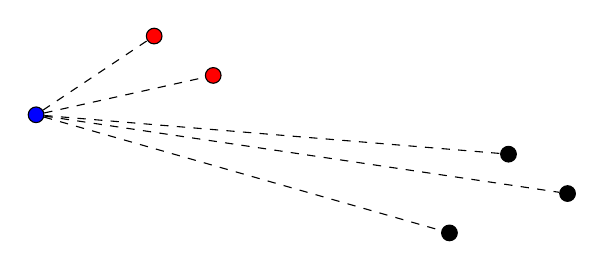
\begin{tikzpicture}[x=1.5cm]
                        \node[inner sep=2pt, circle, draw=black, fill=blue] (test) at (0, 0) {};
                        \node[rbtr] (nn0) at (1, 1) {};
                        \node[rbtr] (nn1) at (1.5, 0.5) {};
                        \node[rbtb] (nn2) at (4, -0.5) {};
                        \node[rbtb] (nn3) at (3.5, -1.5) {};
                        \node[rbtb] (nn4) at (4.5, -1) {};

                        \draw
                        (test) edge[dashed] (nn0)
                        (test) edge[dashed] (nn1)
                        (test) edge[dashed] (nn2)
                        (test) edge[dashed] (nn3)
                        (test) edge[dashed] (nn4);
                    \end{tikzpicture}
                    \hfill
                    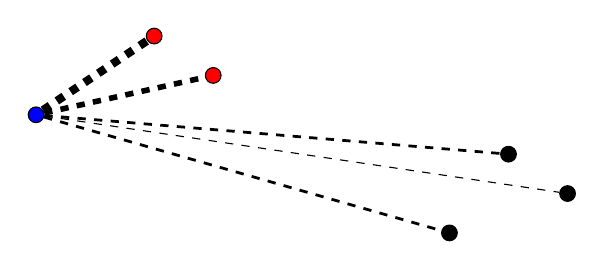
\begin{tikzpicture}[x=1.5cm]
                        \node[inner sep=2pt, circle, draw=black, fill=blue] (test) at (0, 0) {};
                        \node[rbtr] (nn0) at (1, 1) {};
                        \node[rbtr] (nn1) at (1.5, 0.5) {};
                        \node[rbtb] (nn2) at (4, -0.5) {};
                        \node[rbtb] (nn3) at (3.5, -1.5) {};
                        \node[rbtb] (nn4) at (4.5, -1) {};

                        \draw
                        (test) edge[dashed, line width=3pt] (nn0)
                        (test) edge[dashed, line width=2pt] (nn1)
                        (test) edge[dashed, line width=1pt] (nn2)
                        (test) edge[dashed, line width=1pt] (nn3)
                        (test) edge[dashed] (nn4);
                    \end{tikzpicture}
                \end{center}
                The idea is that we add weights to each neighbour (depending on distance), typically a higher weight for closer neighbours.
                We then assign the class based on which class has the largest sum.
                This metric, $w^{(i)}$, is any measure favouring the votes of nearby neighbours, such as;
                \begin{itemize}
                    \itemsep0em
                    \item inverse of distance
                        \[w^{(i)} = \frac{1}{d(x^{(i)}, x^{(q)})}\]
                    \item Gaussian distribution
                        \[w^{(i)} = \frac{1}{\sqrt{2 \pi}}e^{-\frac{d\left(x^{(i)}, x^{(q)}\right)^2}{2}}\]
                \end{itemize}
                The value of $k$ is less important in the weighted case, as distant examples won't greatly affect classification.
                If $k = N$, where $N$ is the size of the training set, it is a global method, otherwise it is a local method (only considering the samples close by).
                This method is also more robust to noisy training data, however it can be slow for large datasets.
                \medskip

                As this method relies on distance metrics, it may not work well if using all features in high dimensional spaces.
                If these features are irrelevant, instances in the same class may be far from each other.
                One solution to this is to weight features differently.
                \medskip

                k-NN can also be used for regression, either by computing the mean value across $k$ nearest neighbours (which leads to a very rough curve), or by using locally weighted regression, which computes the weighted mean value across $k$ nearest neighbours, leading to a smoother curve.
            \subsubsection*{Classification with Decision Trees}
                Decisions trees are the principal of focusing on a subset or single feature of each sample and then make a decision whether it's true or false (for each feature), and repeat this process to finer decisions until we manage to classify the sample that we want to check.
                \medskip

                In decision trees, we learn a succession of linear decision boundaries that we can use to eventually correctly classify samples.
            \subsubsection*{How to select the 'optimal' split rule}
            \subsubsection*{Worked example for construction decision tree}
            \subsubsection*{Summary and other considerations with decision tree}
        \subsection*{Week 4 (Machine Learning Evaluation)}
        \subsection*{Week 5 (Artificial Neural Networks I)}
        \subsection*{Week 6 (Artificial Neural Networks II)}
        \subsection*{Week 7 (Unsupervised Learning)}
        \subsection*{Week 8 (Genetic Algorithms)}
\end{document}